\documentclass[a4paper,10pt]{beamer}
\usepackage[utf8x]{inputenc}
\usepackage[T1]{fontenc}
\usepackage[english]{babel}
\usepackage{hyperref,graphicx,multicol,eurosym,tabularx,color}
\usetheme{Berkeley}

\setbeamertemplate{navigation symbols}{\large \insertframenumber /\inserttotalframenumber}
\newcolumntype{M}[1]{>{\centering\arraybackslash}m{#1}}

\title{3D objects from 2D drawings}
\author[Groupe 3INFO]{Aurélien Fontaine, Manutea Huang, Etienne Geantet, Arnaud Martin}
\institute[INSA de Rennes]{Institut National des Sciences Appliquées de Rennes}
\date{\today}

\begin{document}
	
	\begin{frame}
		\begin{titlepage}
			\centerline{
\includegraphics[scale=0.1]{images/logos/logoINSA.jpg}}
			\centerline{Tutors : François Lehericey and Bertrand Coüasnon}	
		\end{titlepage}
	\end{frame}

	\section{Introduction}

		
		\subsection{Our subject}
		
		\begin{frame}{The subject}
			\begin{itemize}
				\item Create an object from several drawing on a tablet
				%\centerline{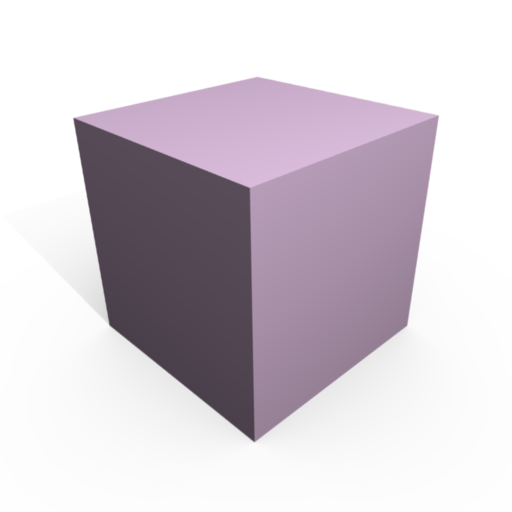
\includegraphics[height=100pt]{images/cube.png}
				%	\mbox{ }
				\item Easy to use: <1min to create a new model
				\item Send this object to a server running Unity (the 3D environment)
			\end{itemize}
			\centerline{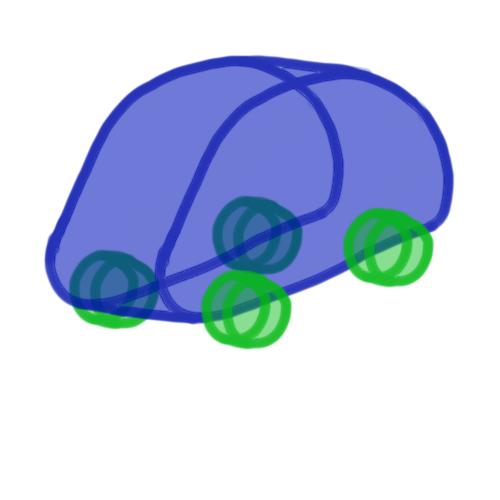
\includegraphics[height=80pt]{images/modelcar.png}}              
			\underline{Final objective :} Create simple models to occupy a 3D environment
		\end{frame}
		
			
	\begin{frame}
		\tableofcontents
	\end{frame}
			
		\subsection{Existing technologies}
		
		\begin{frame}{A project from Sony}
			Project PS4 : The PlayRoom (now available)
			\href{run:Video_intro_playroom.wmv}{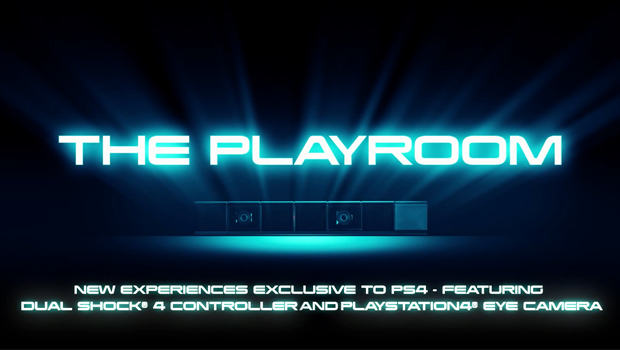
\includegraphics[width=200pt]{images/The-Playroom.jpg}}
			\begin{itemize}
				\item A closed software
				\item Too simple : 1 single drawing = 1 model

			\end{itemize}
		\end{frame}
		
			\begin{frame}{Drawing editors}
				\begin{itemize}
					\item A lot of drawing editors : Markers, LayerPaint, SketchBook, ...
					\item Great drawings but :
					\begin{itemize}
						\item No possibility of making a 3D object
						\item Or very hard to create
					\end{itemize}
					\item Source code inaccessible
				\end{itemize}
			\end{frame}
	
	\section{Our solution}
		\subsection{Specifications}
		
		\begin{frame}{Specifications}
			\begin{itemize}
				\item Android Tablet application
				\item Create more or less complex 3D objects
				\item Ergonomic application :
				\begin{itemize}
					\item Easy to use for a novice user
					\item Fast creations
				\end{itemize}
				\item The exportation: compatible with a Unity server
				\begin{itemize}
					\item Add a plugin to receive the 3D models
				\end{itemize}
			\end{itemize}
			
		\end{frame}
		
		\subsection{The interface}
		
		
			\begin{frame}{The app}
				A \underline{step by step} creation :
				\begin{itemize}
					\item Draw in 2D
					\item Extrusion of our drawing
					\item Placing of the model in a 3D environment
					\item Export to the server
				\end{itemize}
				All that in less than 1 min for a novice user
			\end{frame}
		
		
			\begin{frame}{The app}
				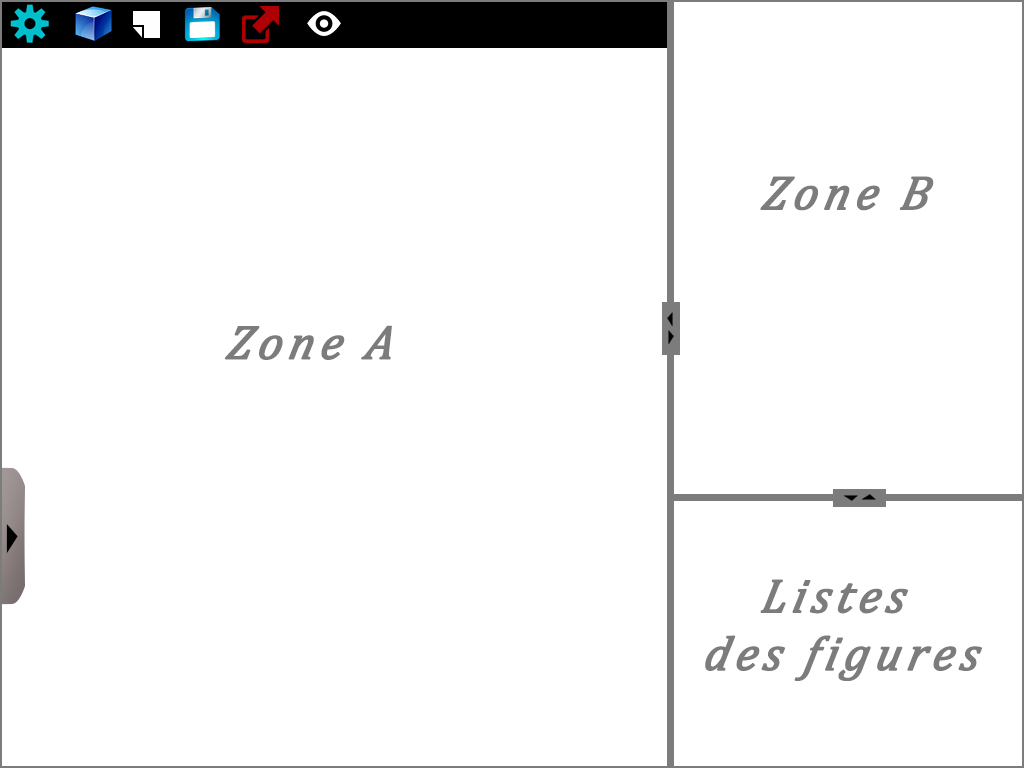
\includegraphics[height=205pt]{maquette/maquette_1.png}
			\end{frame}
			
			\begin{frame}{Areas}
				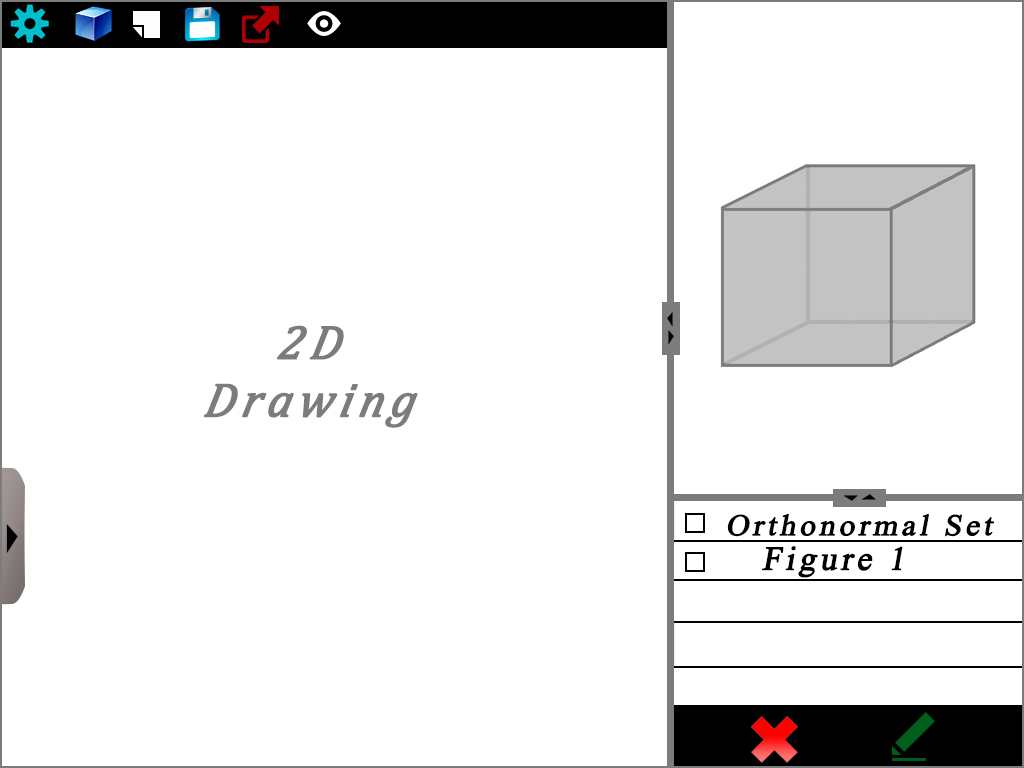
\includegraphics[height=205pt]{maquette/maquette_2.png}
				
				\pause
				
				\underline{Objective:} draw a red cube => put it in the corner
			\end{frame}
			
			\begin{frame}{Draw 2D model}
				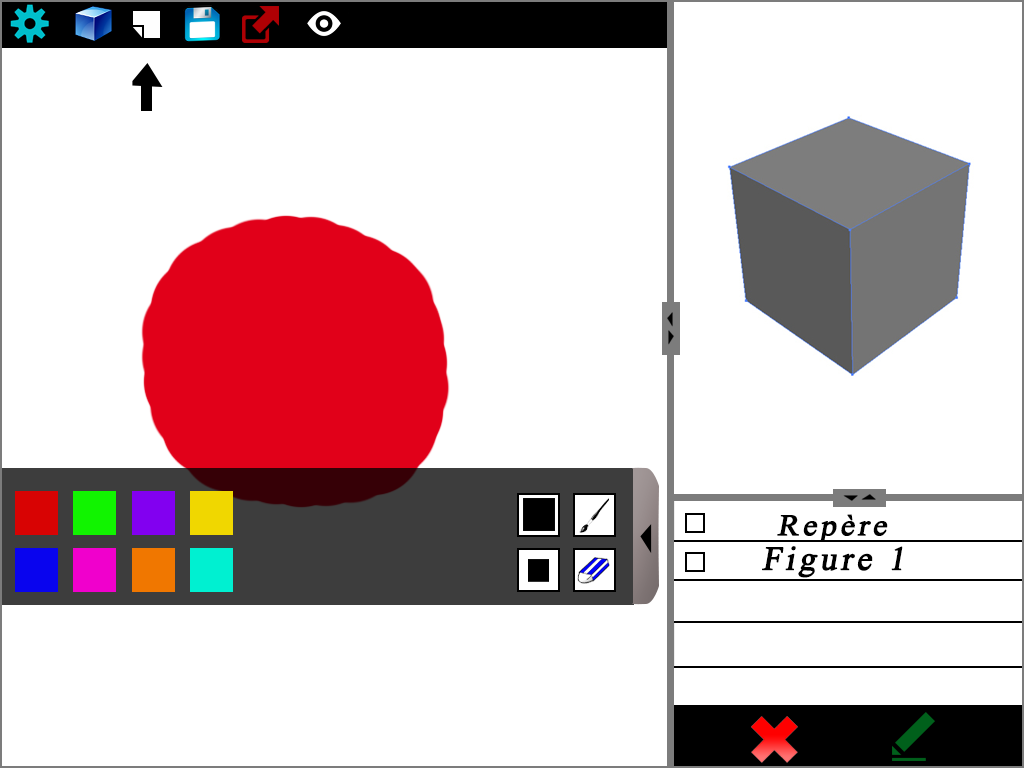
\includegraphics[height=205pt]{maquette/maquette_3.png}
				
				Draw a square
			\end{frame}
			
			\begin{frame}{2D to 3D}
				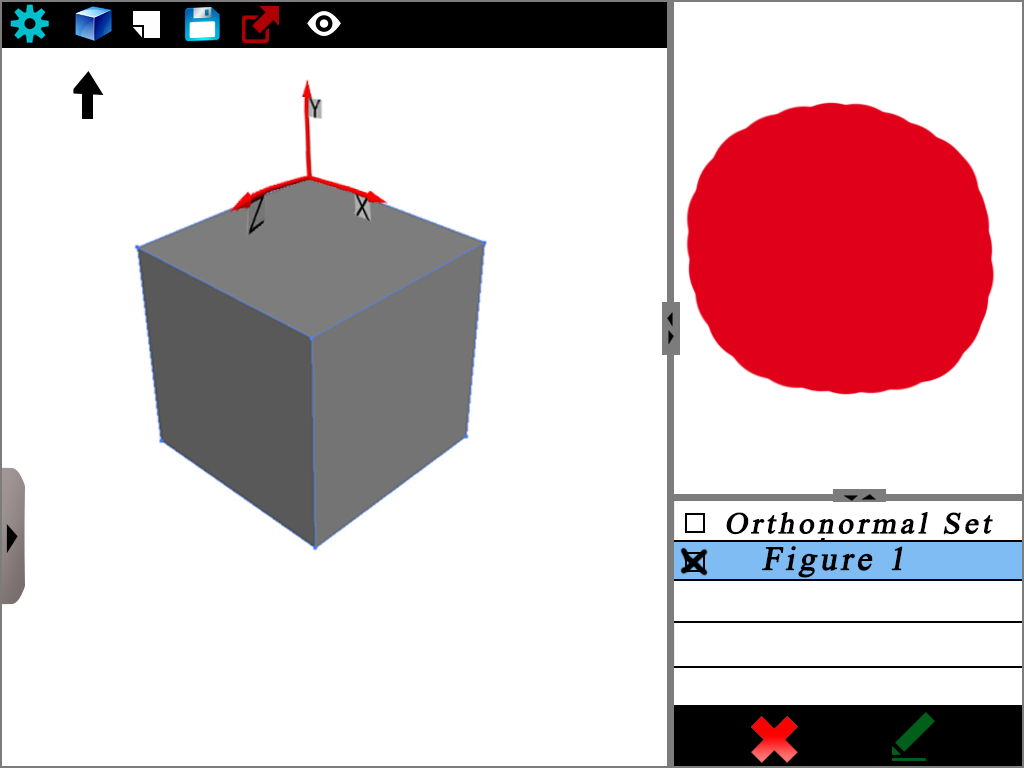
\includegraphics[height=205pt]{maquette/maquette_4.png}
				
				Extrude the square
			\end{frame}
			
			\begin{frame}{Placing in 3D environment}
				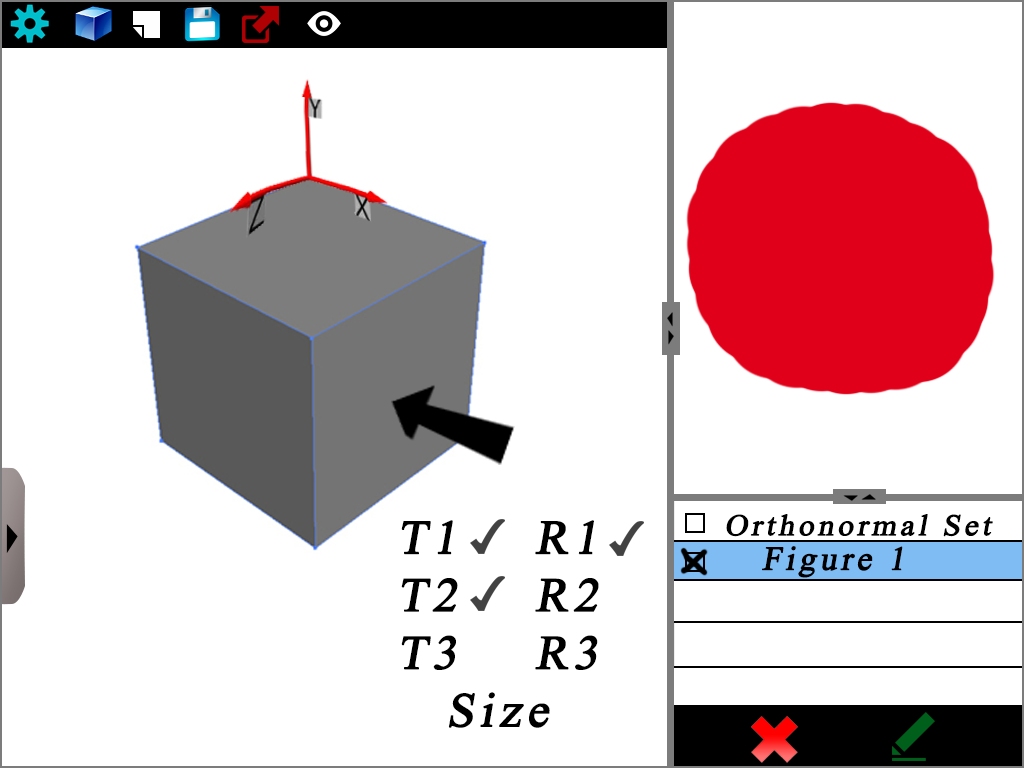
\includegraphics[height=205pt]{maquette/maquette_5.png}
				
				The problem of a 3D placement
			\end{frame}
			
			\begin{frame}{Placing in 3D environment}
				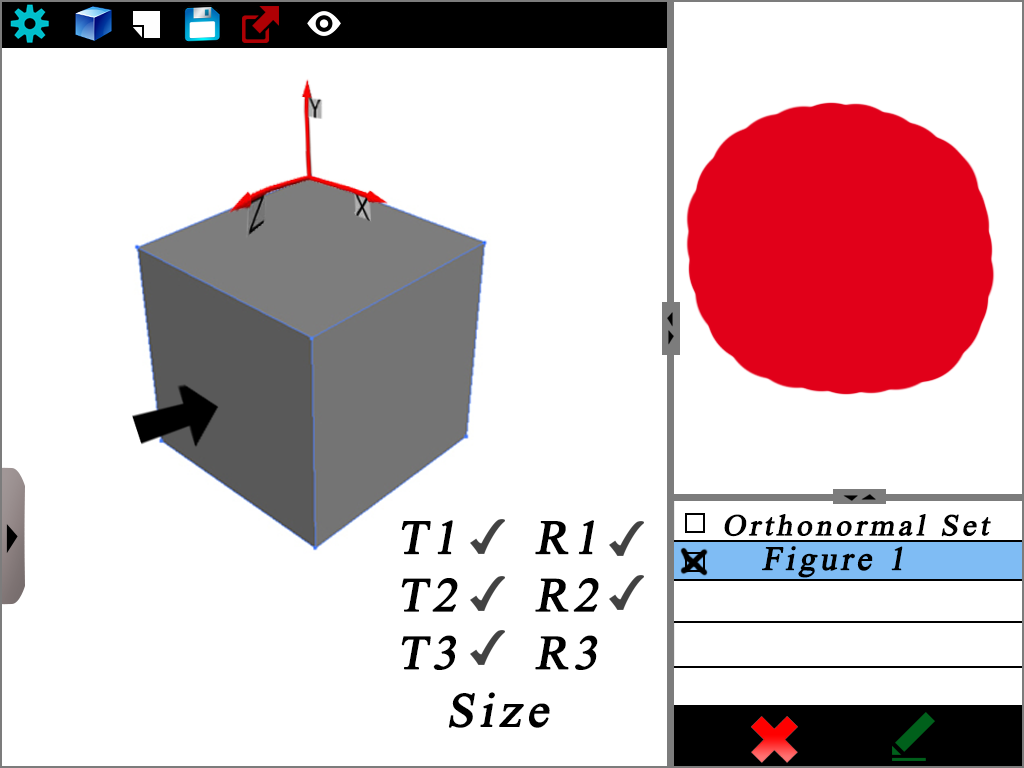
\includegraphics[height=205pt]{maquette/maquette_6.png}
				
				Deplacing our cube on axis X
			\end{frame}
			
			\begin{frame}{Finish placement}
				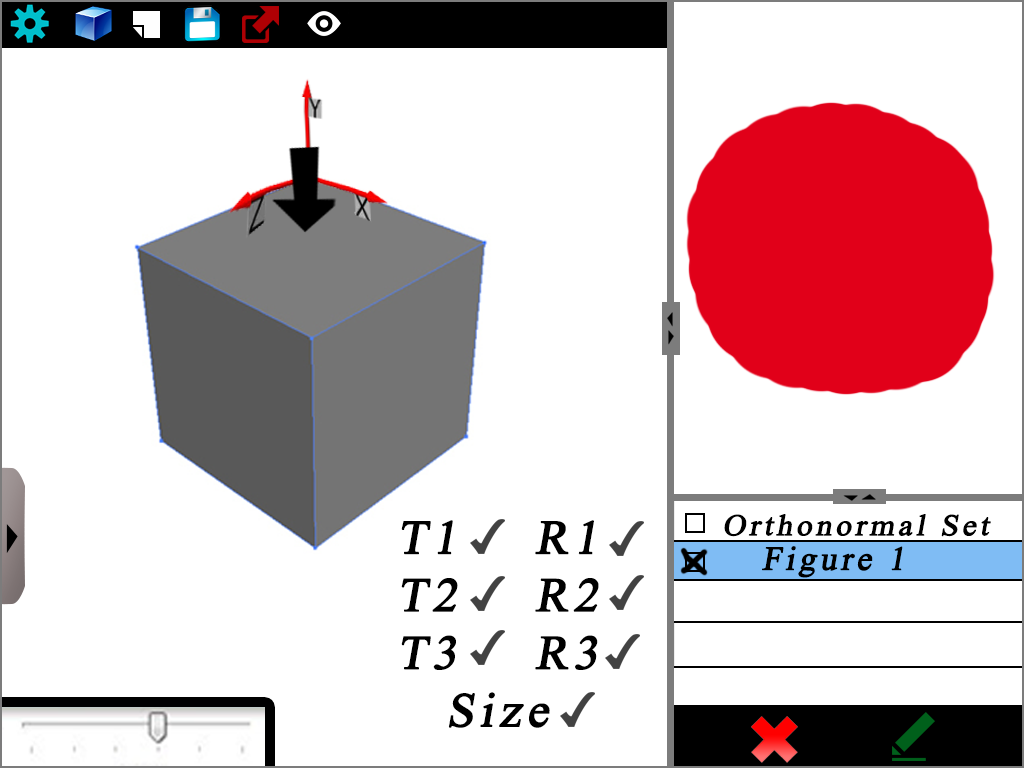
\includegraphics[height=205pt]{maquette/maquette_7.png}
				
				Same for axis Y and Z
			\end{frame}
			
			\begin{frame}{Send to the server}
				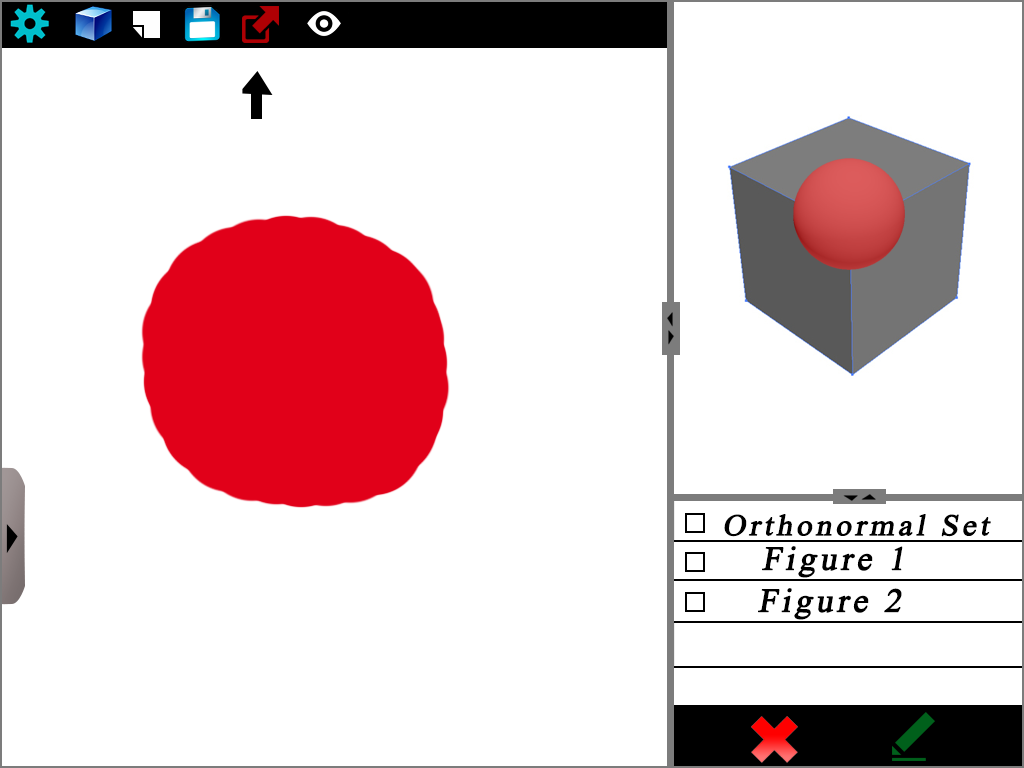
\includegraphics[height=205pt]{maquette/maquette_8.png}
			\end{frame}
			
		
		
	\section{The technology : the engine}
			
			\begin{frame}{The technology}
				How could we make our application ?
				\begin{itemize}
					\item FPS (First-person shooter) game engines
					\item API (Application Programming Interface)

				\end{itemize}
			\end{frame}
			
		\subsection{FPS game engines}
		
			\begin{frame}{Unreal engine}
				\begin{multicols}{2}
				
\includegraphics[height=100pt]{images/logos/Unreal_Engine.png}\\
				
				\columnbreak 
				
				 \begin{itemize}
				 	\item \underline{Use :}\\		
					 FPS game engine	 
					 \item \underline{Qualities :}\\
						 \begin{itemize}
						 	\item Can work with a lot of objects
						 	\item Easy to use : C++
						 \end{itemize}
				 \end{itemize}		 
				\end{multicols}
				\begin{itemize}
					\item \underline{Defaults :}\\
					\begin{itemize}
						\item View FPS inevitable
						\item A sand box for game
						\item Lack of tools to develop on tablets
						\item Licence expensive (19\euro/month + 5\%)
					\end{itemize}
				\end{itemize}
			\end{frame}
			
			\begin{frame}{CryEngine}
				\begin{multicols}{2}
					
\includegraphics[height=100pt]{images/logos/Cry_Engine.png}\\
					
					\columnbreak 
					
					\begin{itemize}
						\item \underline{Use :}\\		
						FPS game engine				
						\item \underline{Qualities :}\\
						\begin{itemize}
							\item Can work with a lot of objects
							\item Easy to use : C++
							\item Cross platform
						\end{itemize}
					\end{itemize}		 
				\end{multicols}
				\begin{itemize}
					\item \underline{Defaults :}\\
					\begin{itemize}
						\item View FPS inevitable
						\item A sand box for game
						\item Lack of tools to develop on tablets
						\item Licence expensive (9.99\euro/month)
					\end{itemize}
				\end{itemize}
			\end{frame}
			
			
		\subsection{Others API}
		
			\begin{frame}{OpenGl}
				\begin{multicols}{2}
					
\includegraphics[height=70pt]{images/logos/OpenGL_logo.png}\\
					
					\columnbreak 
					
					\begin{itemize}
						\item \underline{Use :}\\		
						Hardware oriented API			
						\item \underline{Qualities :}\\
						\begin{itemize}
							\item Need few resources
						\end{itemize}
					\end{itemize}		 
				\end{multicols}
				\begin{itemize}
					\item \underline{Defaults :}\\
					\begin{itemize}
						\item New language
						\item Hard to create a simple object
						\item Hard to move to different devices
						\item OpenGl ES : less functions than OpenGl
					\end{itemize}
				\end{itemize}
			\end{frame}
			
			\begin{frame}{Autodesk Maya}
				\begin{multicols}{2}
					
\includegraphics[height=60pt]{images/logos/Autodesk_Maya.png}\\
					
					\columnbreak 
					
					\begin{itemize}
						\item \underline{Use :}\\		
						3D computer graphics software		
						\item \underline{Qualities :}\\
						\begin{itemize}
							\item Easy to use : C++
							\item Very rich library
						\end{itemize}
					\end{itemize}		 
				\end{multicols}
				\begin{itemize}
					\item \underline{Defaults :}\\
					\begin{itemize}
						\item Very expensive licence (\$185.00/month)
						\item Made for specials effects in films
					\end{itemize}
				\end{itemize}
			\end{frame}
		
			\begin{frame}{Unity}
				\begin{multicols}{2}
					
\includegraphics[height=80pt]{images/logos/Logo_Unity.jpg}\\
					
					\columnbreak 
					
					\begin{itemize}
						\item \underline{Use :}\\		
						Cross-platform game creation system 		
						\item \underline{Qualities :}\\
						\begin{itemize}
							\item Easy to export to an Unity server
							\item Easy to use : C\#
							\item Lots of help for tablet development
							\item Very rich library
							\item Free licence available
						\end{itemize}
					\end{itemize}		 
				\end{multicols}
				\begin{itemize}
					\item \underline{Defaults :}\\
					\begin{itemize}
						\item Paying version for all the features
					\end{itemize}
				\end{itemize}
			\end{frame}
			
			\begin{frame}{A recap}
				\begin{tabular}{|M{50pt}|M{30pt}|M{45pt}|M{80pt}|M{30pt}|}
					\hline
					\textbf{Software} & \textbf{Easy to learn} & \textbf{Manage many objects} & \textbf{Price} & \textbf{Help for tablet}\\
					\hline
					\textit{Unreal Engine} & \color{green}{\checkmark} & \color{green}{\checkmark} &19\euro/month + 5 \% & \color{red}{$\times$}\\
					\hline
					\textit{CryEngine} & \color{green}{\checkmark} & \color{green}{\checkmark} & 9.99\euro/month & \color{orange}{$\sim$}\\
					\hline
					\textit{OpenGl} & \color{red}{$\times$} & $\sim$ & \color{green}{0\euro} & \color{red}{$\times$}\\
					\hline
					\textit{Autodesk Maya} & \color{red}{$\times$} & \color{green}{\checkmark} & \color{red}{\$185.00/month} & $\sim$\\
					\hline
					\textit{Unity} & \color{green}{\checkmark} & \color{green}{\checkmark} & \color{green}{0\euro : free licence} & \color{green}{\checkmark} \\
					\hline
				\end{tabular}
			\end{frame}
			
	\section{Network}
			
			\begin{frame}{Network}
				\centerline{
\includegraphics[height=150pt]{images/network/network.png}}
			\end{frame}
			
		\subsection{How will it work?}
		
			\begin{frame}{What is already set up ?}
					\centerline{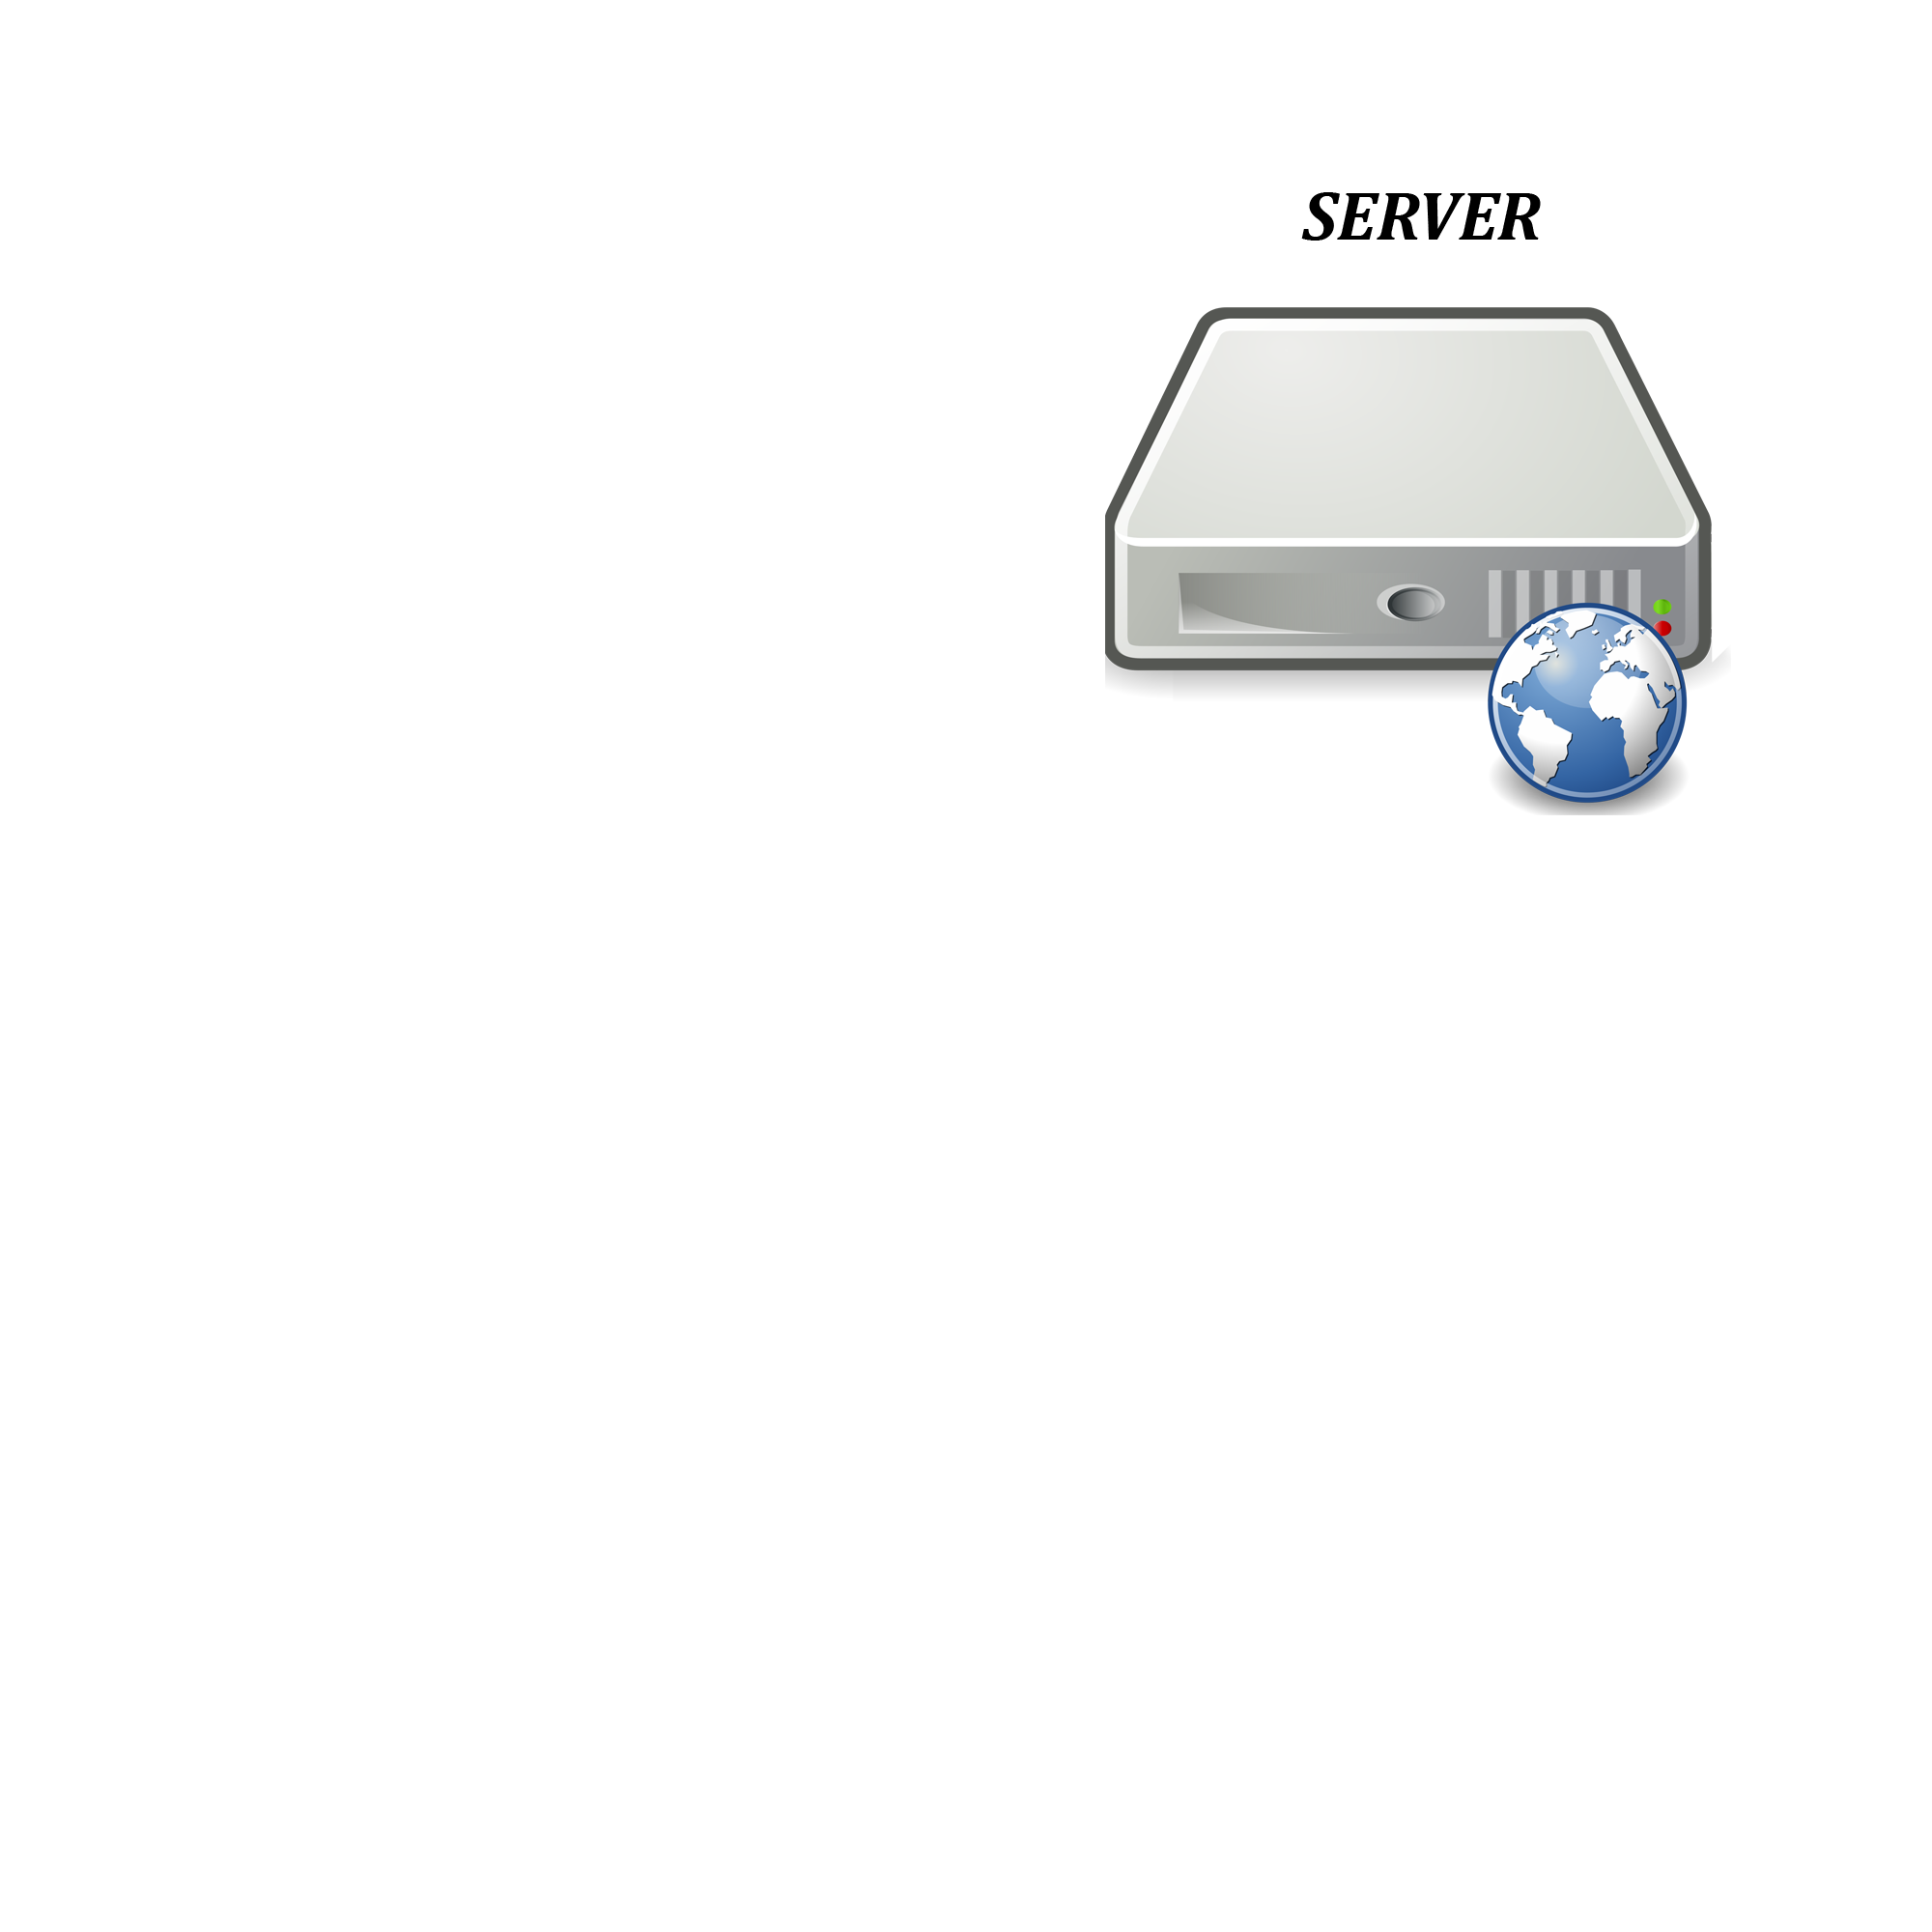
\includegraphics[height=100pt]{images/network/server.png}
					\pause
					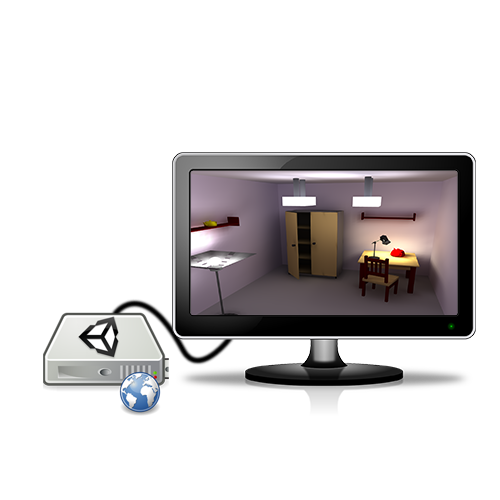
\includegraphics[height=200pt]{images/network/scenebefore.png}}
			\end{frame}
			
			\begin{frame}{The purpose: sending the model}
				\centerline{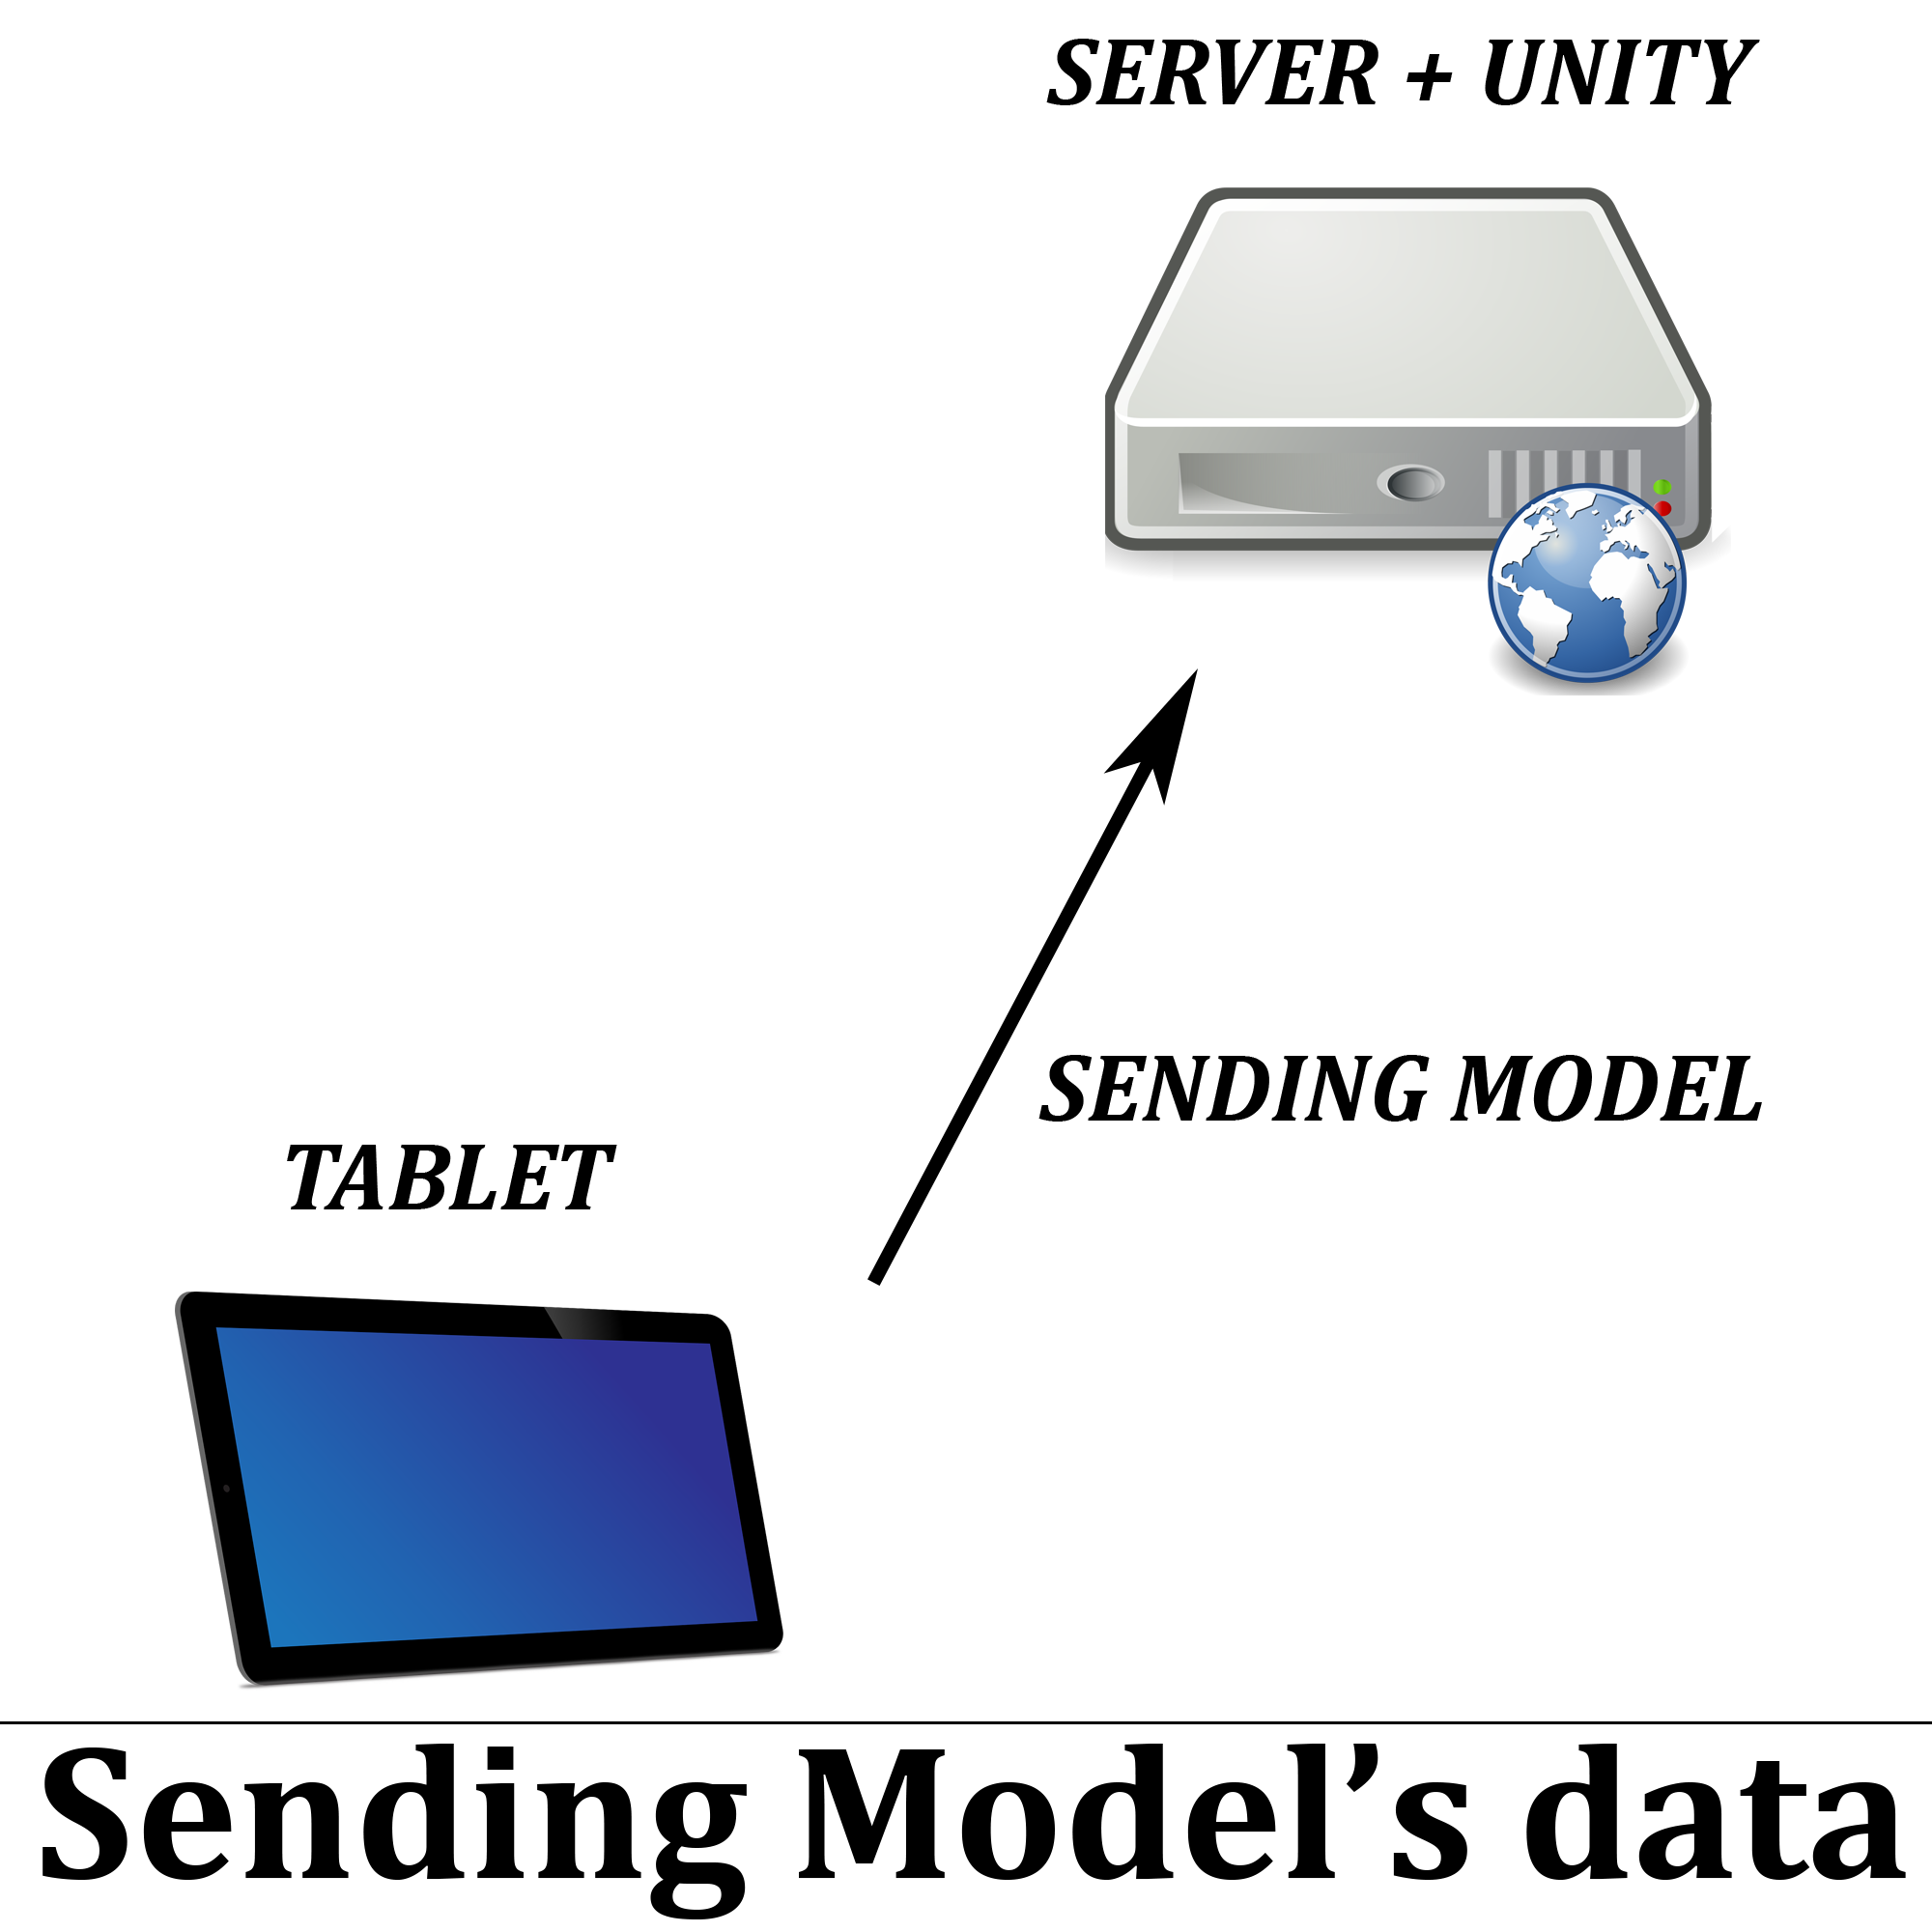
\includegraphics[height=150pt]{images/network/sending_model.png}}
			\end{frame}
			
			\begin{frame}{The purpose: catching the model}
				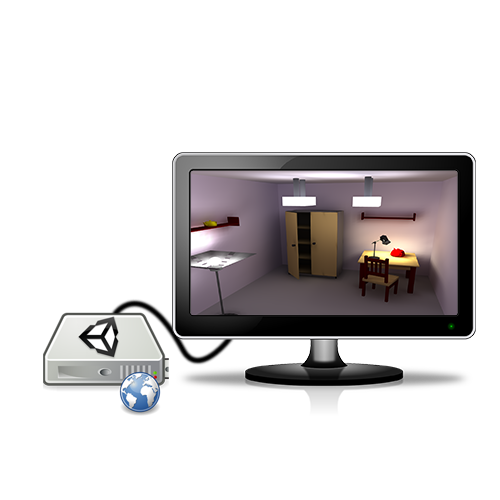
\includegraphics[height=125pt]{images/network/scenebefore.png}
				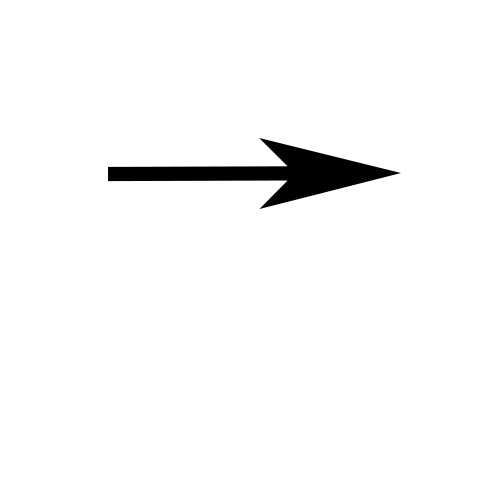
\includegraphics[height=50pt]{images/network/arrow.png}
				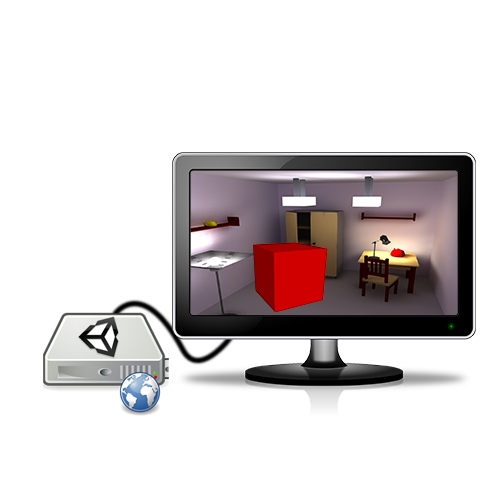
\includegraphics[height=125pt]{images/network/scene.png}
			\end{frame}
			
		\subsection{In the server}
			\begin{frame}{Plugin}
				\centerline{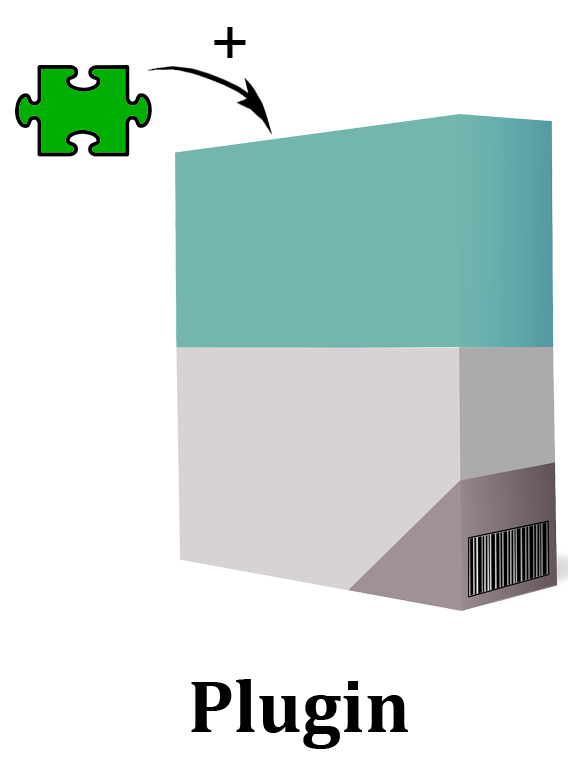
\includegraphics[height=150pt]{images/network/plugin.png}}
				\begin{itemize}	
					\item Little plugin
					\item Only receive data from the tablet
					\item Integrated in the 3D scene
				\end{itemize}	
											
			\end{frame}
			
		\subsection{In the tablet}
			
			\begin{frame}{External Application}
				\begin{multicols}{2}
					
					\begin{itemize}
						\item Use resources
					\end{itemize}
					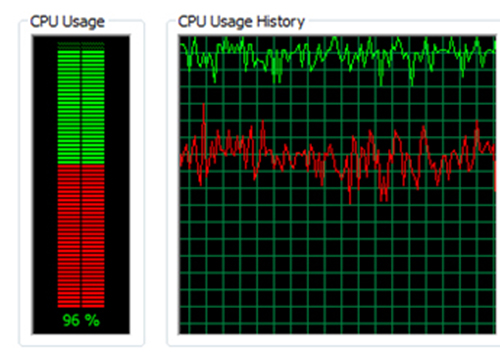
\includegraphics[height=100pt]{images/network/CPU_resources.jpg}
					\pause
					\columnbreak	
					
					\begin{itemize}
						\item Too complex to set up /
						
						 to use
					\end{itemize}
					
\includegraphics[height=100pt]{images/network/complex.png}					
				\end{multicols}	
			\end{frame}
		
			\begin{frame}{What Protocol to use ?}
					\begin{multicols}{2}
						HTTP:
						\begin{itemize}
							\item Use: Get data from a server
							\item Problem: Only post specific files to a server
						\end{itemize}
						\pause
						
						
\includegraphics[height=135pt]{images/network/nmft.png}
						\pause
						
						\columnbreak
						FTP:
						\begin{itemize}
							\item Use: Send files to a server
							\item Problem: Too complex for the user
						\end{itemize}
						\pause
						
						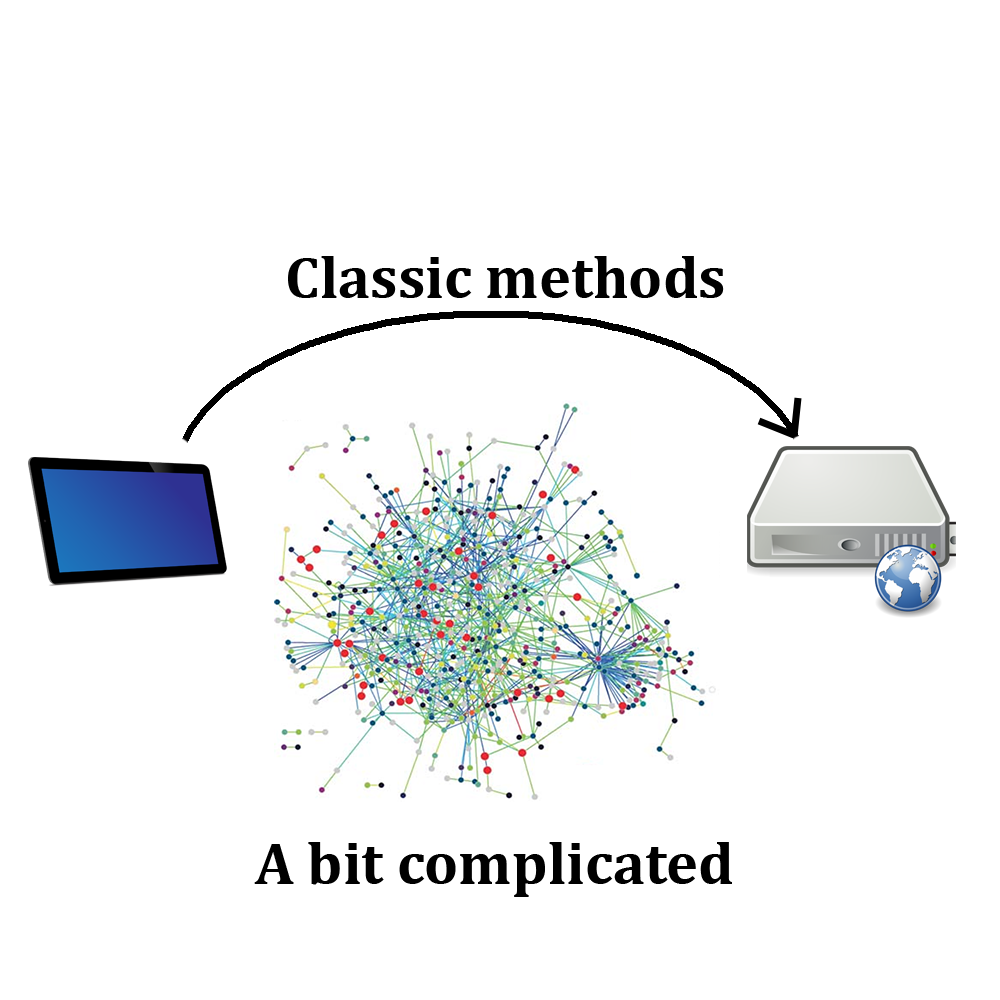
\includegraphics[height=135pt]{images/network/classicnet.png}
					\end{multicols}
					
			\end{frame}
			
		\begin{frame}{Unity Assets}
			\begin{itemize}
				\item Unity Assets : looks like Java Classes
				\item Well implemented
				\item Documentation available
				\pause
				\item \textbf{\underline{Facilitate Unity to Unity Networking}}
				\pause
			\end{itemize}
			\centerline{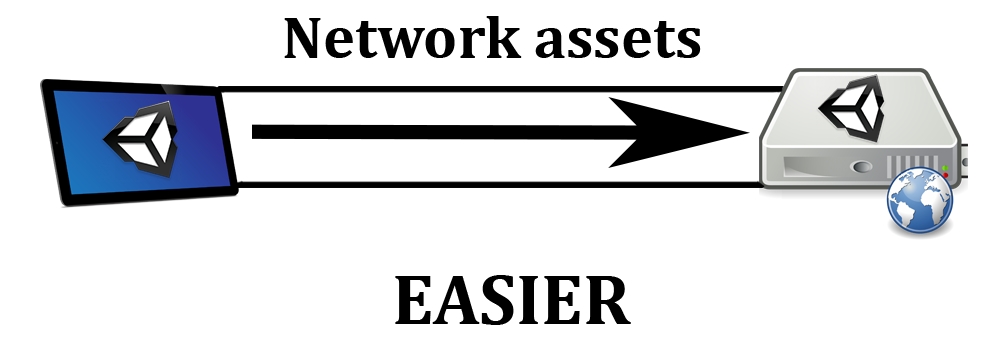
\includegraphics[height=75pt]{images/network/easier.png}}
		\end{frame}
		
		

	
	\section{Conclusion}
	
		\begin{frame}{Conclusion}
			The result of this first research part of our project:
			\hspace{4cm}
			\begin{itemize}
				\item Defined an ergonomic interface for novice users
					\begin{itemize}
						\item Easy and intuitive way to add drawings
						\item Simple steps to assemble our new object with the previous one
					\end{itemize}
					\hspace{3cm}
				\item We looked for the best existing technology
				\hspace{3cm}
				\item Our engine choice : Unity
					\begin{itemize}
						\item Easy to use
						\item Simplified networking
					\end{itemize}
				
			\end{itemize}
		\end{frame}
		
\end{document}
